% Section 1.1: self-contained derivation, figures and NumPy companion.
\section{Recap of Logistic Regression}
\label{sec:logreg_to_mlp:recap_of_logistic_regression}

\begin{keyidea}[The question behind every formula]
A classifier must decide what to do, but first it can estimate what might be true.
Logistic regression separates these two tasks: a model assigns a probability to a
binary outcome, and a decision rule turns that probability into an action.
The sigmoid specifies the probability model; cross-entropy measures how much
probability that model assigned to the outcome actually observed.
\end{keyidea}

\subsection{The problem: a decision is not a probability}
Imagine a robot about to grasp a cup. From its camera and estimated gripper pose,
it measures a centering error and an angular misalignment. The outcome is
$Y=1$ for a successful grasp and $Y=0$ for a failure. We would like to answer
both ``How likely is success?'' and ``Should the robot attempt this grasp?''
These are different questions. A success probability of $0.7$ might justify a
cheap retryable grasp but not a grasp whose failure breaks an expensive object.

Why not just fit a line to the labels? A real-valued affine prediction can be
negative or greater than one. Why not immediately threshold that line? A hard
threshold throws away the distinction between a barely positive score and a
strongly positive score. It also gives a piecewise constant classification error,
which offers little useful gradient information. We therefore seek a smooth
conditional probability model before choosing a decision rule.

This section develops the connected chain
\[
\text{features}\longrightarrow\text{score}\longrightarrow\text{probability}
\longrightarrow\text{likelihood}\longrightarrow\text{loss}
\longrightarrow\text{learning and decisions}.
\]
We first understand a fixed model. Only later do we vary its parameters to train
it. The examples and plots here are constructed teaching examples, not empirical
claims about a deployed robot.

\subsection{Notation and the assumptions we are making}
Let $x=(x_1,\ldots,x_d)^\top\in\mathbb R^d$ denote the measured features and let
$Y\in\{0,1\}$ be a random outcome. Define the augmented input and parameter vector
\[
\tilde x=\begin{bmatrix}1\\x\end{bmatrix}\in\mathbb R^{d+1},\qquad
w=\begin{bmatrix}b\\a\end{bmatrix},\qquad
z=w^\top\tilde x=b+a^\top x.
\]
The slides call the bias $w_0$ and use $x_0=1$; thus their $w^\top x$ is our
$w^\top\tilde x$. We keep the tilde to distinguish the actual feature space from
the augmented space. The scalar $z$ is the \emph{score} or \emph{logit}.

\begin{center}
\begin{tabular}{ll}
\toprule
Symbol & Meaning \\
\midrule
$Y$ & Random binary label before observing the outcome \\
$y$ & Observed label, exactly zero or one \\
$q(x)$ & True conditional probability $\Pr(Y=1\mid X=x)$ \\
$p_w(x)$ & Model probability, also written $h_w(x)$ \\
$\hat y$ & In the slides, the probability $h_w(x)$ \\
$\hat c$ & Hard class prediction, zero or one \\
$\ell(p,y)$ & Loss on one observation \\
$J(w)$ & Mean loss over the training data \\
\bottomrule
\end{tabular}
\end{center}

\paragraph{Definitions, assumptions, consequences.}
That a binary conditional distribution is Bernoulli is a consequence of its two
possible outcomes: it is completely specified by one probability. That its
\emph{log-odds is affine in the chosen features} will be our modeling assumption.
That independent observations give a product likelihood is an additional
sampling assumption. Cross-entropy then follows from maximum likelihood; its
convexity follows from calculus. These statements play different logical roles.

Conditioning matters. We model $Y\mid X=x$, not one identical Bernoulli law for
all inputs. At different inputs the success probabilities can differ. Treating
$Y$ probabilistically does not assert that the world is fundamentally random.
Unmeasured friction, occlusion, noisy sensors, or missing features can make an
outcome unpredictable from the information we have.

\subsection{Inventing the sigmoid through odds and evidence}
A useful probability must stay in $[0,1]$, while a linear score can take any real
value. Many maps could enforce this range. Why use this particular one?

For $0<p<1$, define the \emph{odds} as $p/(1-p)$. If $p=0.8$, the odds are $4$:
success has four times the probability of failure. Odds live in $(0,\infty)$;
logarithms turn this into the whole real line. The \emph{log-odds} is
\[
\operatorname{logit}(p)=\log\frac{p}{1-p}.
\]
We now \emph{assume} that evidence measured in log-odds is additive:
\begin{equation}
\log\frac{p_w(x)}{1-p_w(x)}=b+\sum_{j=1}^d a_jx_j=z.
\label{eq:lr11-logodds}
\end{equation}
Solving, rather than memorizing, gives
\[
\frac{p}{1-p}=e^z
\quad\Longrightarrow\quad p=e^z(1-p)
\quad\Longrightarrow\quad p(1+e^z)=e^z
\quad\Longrightarrow\quad
\boxed{p_w(x)=\sigma(z)=\frac{1}{1+e^{-z}}.}
\]
This is an equivalence: affine log-odds and a sigmoid of an affine score describe
exactly the same model. Binary labels alone do not force this choice; a probit
link, for example, would define a different model.

Equation~\eqref{eq:lr11-logodds} also explains the parameters. Increasing $x_j$ by
one unit with other features held fixed multiplies the odds by $e^{a_j}$.
It does \emph{not} add $a_j$ to the probability. The bias is the log-odds at
$x=0$, so $p_w(0)=\sigma(b)$. This interpretation depends on units and on whether
zero is meaningful for the features.

\paragraph{Why additive log-odds is a reasonable idea.}
Bayes' rule gives, wherever the densities are positive,
\[
\log\frac{\Pr(Y=1\mid x)}{\Pr(Y=0\mid x)}
=\log\frac{\Pr(Y=1)}{\Pr(Y=0)}
 +\log\frac{p(x\mid Y=1)}{p(x\mid Y=0)}.
\]
Under conditional independence of features, the last term becomes a sum of
featurewise log-likelihood ratios. This motivates adding evidence. Logistic
regression itself does \emph{not} require conditional feature independence; it
models the final conditional log-odds directly. This is a conceptual motivation,
not a claim about the historical invention of the method.

\paragraph{A nontrivial case where the affine assumption is exact.}
Suppose $X\mid Y=k\sim\mathcal N(\mu_k,\Sigma)$, with the same positive-definite
covariance for both classes and priors $\pi_k>0$. The normalizing constants cancel
in the density ratio, leaving
\begin{align*}
\log\frac{q(x)}{1-q(x)}
&=\log\frac{\pi_1}{\pi_0}
-\frac12(x-\mu_1)^\top\Sigma^{-1}(x-\mu_1)
+\frac12(x-\mu_0)^\top\Sigma^{-1}(x-\mu_0)\\
&=(\mu_1-\mu_0)^\top\Sigma^{-1}x
-\frac12\bigl(\mu_1^\top\Sigma^{-1}\mu_1
             -\mu_0^\top\Sigma^{-1}\mu_0\bigr)
+\log\frac{\pi_1}{\pi_0}.
\end{align*}
The quadratic terms in $x$ cancel. Thus a Gaussian generative assumption can
produce precisely a logistic conditional model. Unequal covariances generally
leave quadratic terms. Logistic regression need not fit either Gaussian density
to learn an affine log-odds model.

\subsection{Geometry: why the boundary is a line}
For equal costs of the two mistakes, predict class one when $p_w(x)\geq 1/2$.
To understand its geometry, differentiate:
\[
\sigma'(z)=\frac{e^{-z}}{(1+e^{-z})^2}
=\sigma(z)\bigl(1-\sigma(z)\bigr)>0
\quad\text{for finite }z.
\]
The sigmoid is strictly increasing and $\sigma(0)=1/2$. Therefore
\begin{equation}
\hat c=\mathbf 1\{p_w(x)\geq 1/2\}
=\mathbf 1\{b+a^\top x\geq0\}.
\label{eq:lr11-boundary}
\end{equation}
Its decision boundary is $b+a^\top x=0$. In two dimensions this is a line; in
three, a plane; in $d$ dimensions, a hyperplane, provided $a\ne0$.
Strictly, $b+a^\top x$ is \emph{affine} in $x$ and linear in $\tilde x$.
The informal phrase ``linear classifier'' includes an affine bias.

For the slide's $w=(-3,1,1)^\top$, we obtain
\[
z=-3+x_1+x_2,\qquad x_2=3-x_1.
\]
At $(1,1)$ the score is $-1$ and $p\approx0.269$; at $(1,2)$ it is $0$ and
$p=0.5$; at $(2,2)$ it is $1$ and $p\approx0.731$; at $(4,4)$ it is $5$ and
$p\approx0.9933$. We use class one for ties by convention. Another tie convention
changes only points exactly on the boundary.

\paragraph{Direction, distance, and confidence.}
Moving by a displacement $v$ changes the score by $a^\top v$. If $a^\top v=0$,
we remain on a constant-score hyperplane. Thus $a$ is normal to the boundary.
For $a\ne0$ the signed perpendicular distance from $x$ to the boundary is
\[
\delta(x)=\frac{b+a^\top x}{\|a\|_2},\qquad
p_w(x)=\sigma\bigl(\|a\|_2\delta(x)\bigr).
\]
The score is a \emph{scaled} distance, not a distance in physical units. Scaling
all weights by $c>0$ preserves the boundary but changes the probabilities to
$\sigma(cz)$. As $c$ grows, predictions away from the boundary approach zero or
one. The same classification accuracy can hide very different probability
quality. If $c<0$, the boundary stays but class assignments reverse.

\begin{figure}[htbp]
\centering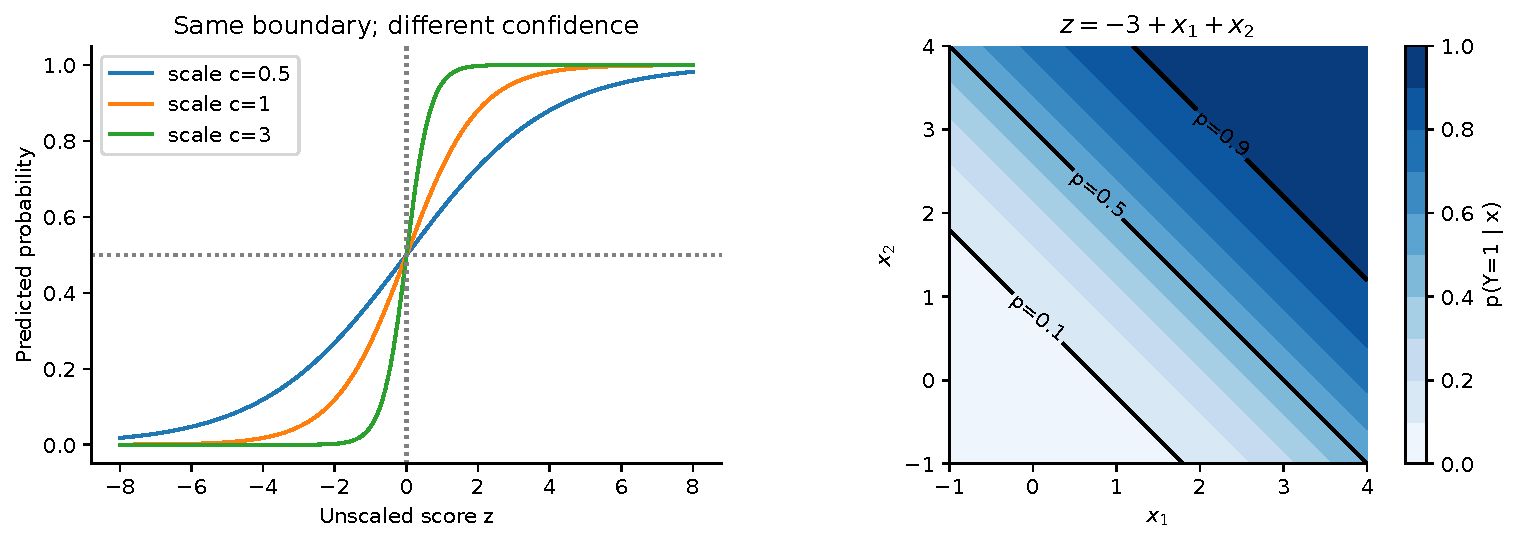
\includegraphics[width=\linewidth]{logreg_1_1/geometry.pdf}
\caption{Left: rescaling a logit changes confidence without moving the zero
threshold. Right: parallel probability contours around the boundary
$x_1+x_2=3$. The sigmoid bends the probability response, not this boundary.}
\label{fig:lr11-geometry}
\end{figure}

\paragraph{Edge cases.}
If $a=0$ and $b\ne0$, the prediction is constant and there is no boundary.
If $a=0$ and $b=0$, every point has probability $1/2$. The normalized-distance
formula cannot be used in either case.

\subsection{What does ``maximally uncertain'' actually mean?}
For a fixed model $w$, $p_w(x)$ is a deterministic number at a fixed input.
It specifies a distribution over $Y$, not a random choice of weights. The model's
Bernoulli variance is
\[
\operatorname{Var}(Y\mid x;w)=p(1-p)=\frac14-(p-\tfrac12)^2,
\]
which is largest at $p=1/2$. Its predictive entropy, in nats, is
\[
H(p)=-p\log p-(1-p)\log(1-p).
\]
Differentiation gives
\[
H'(p)=\log\frac{1-p}{p},\qquad
H''(p)=-\frac1p-\frac1{1-p}<0.
\]
So entropy has a unique maximum $H(1/2)=\log2$. This is the precise sense in which
the model is maximally uncertain at its $0.5$ boundary.

\begin{warning}
A fitted logistic probability is not a guarantee of correctness. A probability
near one may be unjustified on inputs unlike the training data. Predictive
Bernoulli entropy does not separately measure uncertainty about the fitted
parameters, missing model structure, or distribution shift. A decision boundary
at a cost-dependent threshold other than $0.5$ is not a maximum-entropy contour.
\end{warning}

\subsection{Nonlinear boundaries without nonlinear parameters}
Replace raw features with a fixed map $\phi(x)$ and set
$p_w(x)=\sigma(b+a^\top\phi(x))$. The boundary is affine in feature space, but
can be curved in the original coordinates. For example,
\[
\phi(x)=\begin{bmatrix}x_1^2\\x_2^2\end{bmatrix},\qquad
z=4(x_1^2+x_2^2-1).
\]
The $0.5$ boundary is the circle $x_1^2+x_2^2=1$; outside it the model predicts
class one. In $(\phi_1,\phi_2)$ coordinates it is the line
$\phi_1+\phi_2=1$. This is logistic regression with nonlinear basis functions.
The score remains linear in its trainable coefficients.

A second example is XOR on $x_1,x_2\in\{-1,1\}$, with class one for opposite
signs. A feature $x_1x_2$ allows the score $z=-k x_1x_2$, $k>0$, which separates
all four points. An affine score in $x_1,x_2$ alone cannot: the midpoint of the
two class-one points and the midpoint of the two class-zero points are both the
origin, contradicting strict separation by an affine function.

\begin{figure}[htbp]
\centering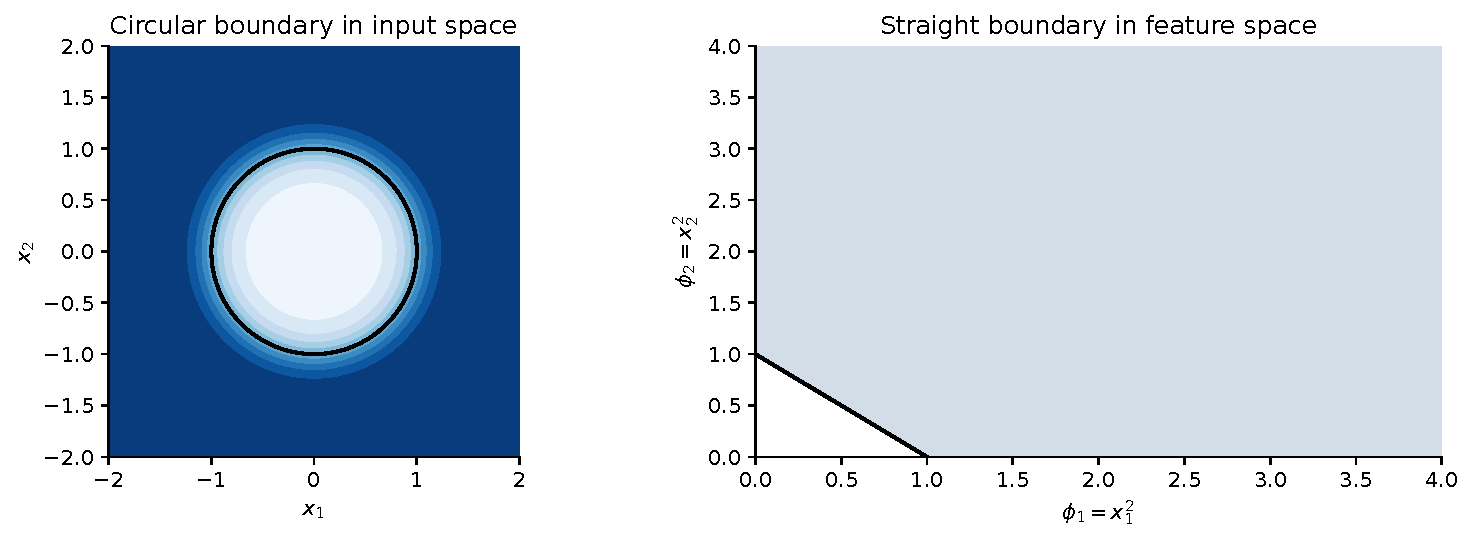
\includegraphics[width=\linewidth]{logreg_1_1/nonlinear_features.pdf}
\caption{One model viewed in two coordinate systems. The curved boundary in
input space becomes straight after the fixed feature transformation. Only the
nonnegative quadrant is reachable in this feature space.}
\end{figure}

\subsection{From a probability model to the likelihood of an observation}
Once an input $x$ is fixed, a Bernoulli model assigns
\[
p_w(Y=y\mid x)=
\begin{cases}p_w(x),&y=1,\\1-p_w(x),&y=0.\end{cases}
\]
Because $y$ is binary, the two cases can be encoded as
\begin{equation}
p_w(Y=y\mid x)=p_w(x)^y\bigl(1-p_w(x)\bigr)^{1-y}.
\label{eq:lr11-bernoulli}
\end{equation}
Check both values: when $y=1$, the second exponent is zero; when $y=0$, the first
is zero. The formula does not make the label continuous. It uses the label as a
selector of the probability assigned to the observed event.

\paragraph{Probability versus likelihood.}
With $w$ fixed, this expression is a probability distribution over $y$; its two
values sum to one. After observing $(x,y)$, the very same expression viewed as a
function of $w$ is a \emph{likelihood}. It asks which parameter choices would
make the observed outcome plausible. It is not a probability distribution over
$w$ and need not integrate to one over parameter space. A Bayesian posterior over
$w$ would additionally require a prior and normalization.

For example, if a grasp succeeds, a model predicting $p=0.9$ assigns likelihood
$0.9$, while one predicting $p=0.2$ assigns $0.2$. If that grasp fails, the
likelihoods reverse their preference: $0.1$ versus $0.8$. A model is judged by
what it said about the event that happened, not just by the thresholded class.

\subsection{Deriving the training objective from maximum likelihood}
Let $\mathcal D=\{(x_n,y_n)\}_{n=1}^N$ and $p_n=p_w(x_n)$. Assume the labels are
conditionally independent across observations given their inputs and the common
parameter $w$. An i.i.d. sample of pairs is a familiar sufficient setup. Then
\[
\mathcal L(w;\mathcal D)=\prod_{n=1}^N
p_n^{y_n}(1-p_n)^{1-y_n}.
\]
The product is a joint conditional probability of the observed labels. Adjacent
video frames or repeated trials on the same object can violate the independence
assumption. The sum loss can still be used as an objective in that case, but the
simple independent-data likelihood interpretation and effective sample size need
care.

We maximize this likelihood. Since $\log$ is strictly increasing, it preserves
which positive value is largest. Since $\log(ab)=\log a+\log b$, it converts
products into sums:
\begin{align*}
\argmax_w\mathcal L(w;\mathcal D)
&=\argmax_w\log\mathcal L(w;\mathcal D)\\
&=\argmax_w\sum_{n=1}^N
\bigl[y_n\log p_n+(1-y_n)\log(1-p_n)\bigr]\\
&=\argmin_w\left\{-\frac1N\sum_{n=1}^N
\bigl[y_n\log p_n+(1-y_n)\log(1-p_n)\bigr]\right\}.
\end{align*}
Negation turns maximization into minimization. Dividing by positive $N$ does not
change the minimizers; it expresses an average per observation. It does change
gradient magnitudes, so the same numerical learning rate need not behave the
same for sum and mean losses.

\begin{definition}[Binary cross-entropy]
For one observation,
\begin{equation}
\boxed{\ell(p,y)=-y\log p-(1-y)\log(1-p).}
\label{eq:lr11-bce}
\end{equation}
For a dataset, the mean negative log-likelihood is
\begin{equation}
\boxed{J(w)=\frac1N\sum_{n=1}^N\ell(p_w(x_n),y_n).}
\label{eq:lr11-mean}
\end{equation}
All logarithms in this section are natural, so losses are measured in nats.
\end{definition}

The brackets in \eqref{eq:lr11-mean} matter: the minus sign applies to both
label-dependent log terms. Changing the logarithm base only multiplies the
objective by a positive constant, leaving its minimizers unchanged.

\subsection{Why a logarithmic penalty makes sense}
The quantity $-\log r$ measures the \emph{surprise} of an event to which the model
assigned probability $r$. An event assigned probability one produces no surprise;
an event assigned a tiny probability produces a large surprise. For independent
events, surprise adds because their probabilities multiply. This is why the
negative logarithm is so natural for a joint probability objective.

\begin{center}
\begin{tabular}{rrrr}
\toprule
Probability of observed outcome $r$ & $0.9$ & $0.5$ & $0.01$\\
\midrule
Surprise $-\log r$ & $0.1054$ & $0.6931$ & $4.6052$\\
\bottomrule
\end{tabular}
\end{center}

For $y=1$, $\ell=-\log p$ decreases as $p$ increases, and
$\partial\ell/\partial p=-1/p$. For $y=0$, $\ell=-\log(1-p)$ increases with $p$,
and $\partial\ell/\partial p=1/(1-p)$. A confidently wrong prediction is much
more expensive than an uncertain one. Correct classification alone does not
make the loss zero: $p=0.51$ and $p=0.99$ both predict one, but their losses for
$y=1$ are about $0.673$ and $0.010$.

\begin{figure}[htbp]
\centering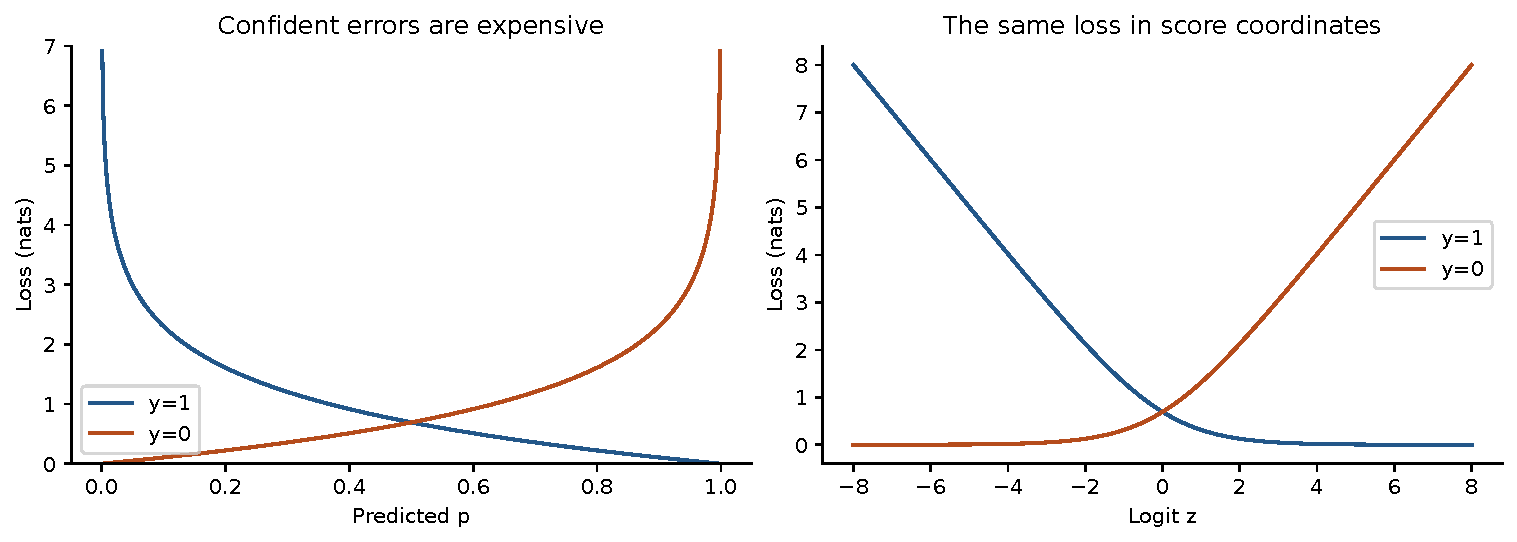
\includegraphics[width=\linewidth]{logreg_1_1/bce.pdf}
\caption{Cross-entropy in probability coordinates (left) and logit coordinates
(right). The probability loss diverges at a wrong endpoint. In logit coordinates
the wrong-direction loss grows approximately linearly for large magnitude.}
\end{figure}

\paragraph{The lecture's two-prediction question.}
For labels $(0,1)$, prediction $(1,1)$ assigns zero joint probability to the
observed data. Its mean BCE is infinite, because the first observation has
$-\log(1-1)=+\infty$. Prediction $(0.5,0.5)$ assigns joint probability $0.25$,
and its mean loss is $-\tfrac12\log(0.25)=\log2\approx0.6931$.
Cross-entropy therefore prefers the second prediction. Exact endpoints are not
produced by a finite mathematical logit, but can occur through rounding. With
$(1-\varepsilon,1-\varepsilon)$ instead, the mean loss is
$-\tfrac12\log[\varepsilon(1-\varepsilon)]$, which diverges as
$\varepsilon\downarrow0$. At an endpoint, interpret zero-weight log terms by
limits; do not compute $0\log0$ directly in floating-point code.

\subsection{Why the best probability is honest, not always extreme}
For a single observed positive label the loss prefers $p\to1$. Does this mean
training should always produce extreme probabilities? Consider repeated outcomes
at the same input with true success probability $q$. The \emph{expected} loss of
reporting $p$ is
\[
r(p;q)=-q\log p-(1-q)\log(1-p).
\]
For $0<q<1$,
\[
\frac{\partial r}{\partial p}
=-\frac{q}{p}+\frac{1-q}{1-p}
=\frac{p-q}{p(1-p)}.
\]
It is negative for $p<q$, zero for $p=q$, and positive for $p>q$. Hence the unique
minimum is the true conditional probability $p=q$. For $q=0$ or $1$, the minimum
is at the corresponding endpoint, approached as a limit by finite logits.
This property is called a \emph{strictly proper scoring rule}.

Suppose ten otherwise identical conditions yield seven successes and three
failures. Their mean loss is $-0.7\log p-0.3\log(1-p)$, minimized at $p=0.7$,
with logit $\log(7/3)\approx0.8473$. Memorizing the latest outcome is not the same
as modeling the underlying probability.

The irreducible minimum is
$r(q;q)=H(q)$, and the excess expected loss is
\[
r(p;q)-H(q)
=q\log\frac{q}{p}+(1-q)\log\frac{1-q}{1-p}
=D_{\mathrm{KL}}\bigl(\operatorname{Bern}(q)\,\|\,
\operatorname{Bern}(p)\bigr)\geq0.
\]
The nonnegativity also follows from the minimization just proved. This gives a
bridge to Section 1.2: cross-entropy is entropy plus the cost of using the wrong
probabilities. A one-hot observed label is an empirical point mass, whose
cross-entropy with the model is precisely the single-observation negative
log-likelihood.

\begin{figure}[htbp]
\centering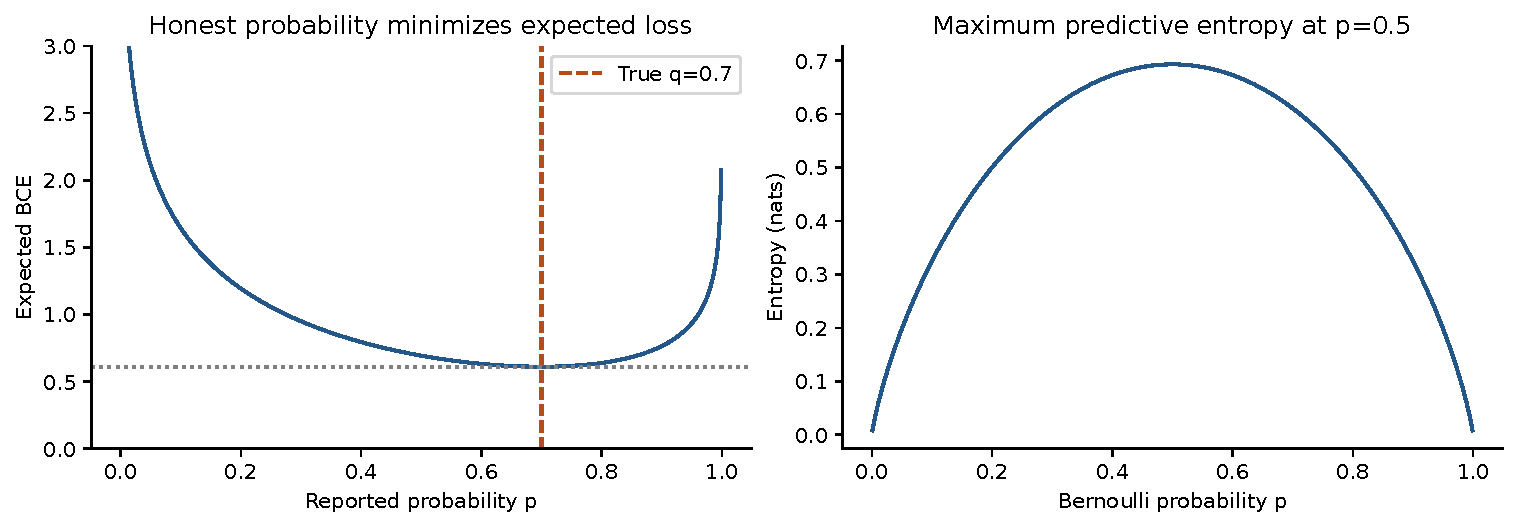
\includegraphics[width=\linewidth]{logreg_1_1/probability_meaning.pdf}
\caption{Left: when the true success frequency is $0.7$, reporting $0.7$ minimizes
expected loss. The dotted horizontal line is the irreducible entropy. Right:
entropy peaks at $0.5$, quantifying uncertainty in a Bernoulli prediction.}
\end{figure}

\paragraph{Empirical versus population risk.}
Training minimizes a sample average. The quantity we ultimately care about is
\[
R(w)=\mathbb E_{X,Y}[\ell(p_w(X),Y)]
=\mathbb E_X\!\left[-q(X)\log p_w(X)
-(1-q(X))\log(1-p_w(X))\right].
\]
This follows by first averaging over the two values of $Y$ at each fixed $X$,
then averaging over inputs. The weights are fixed while this expectation is
evaluated; they vary when comparing models during optimization. Finite data,
misspecified affine log-odds, and distribution shift can keep $p_w$ far from $q$.
A proper loss encourages honest probabilities in the population; it does not
promise that every fitted finite-sample model is calibrated.

\subsection{Deriving the gradient: why the residual is \texorpdfstring{$p-y$}{p-y}}
We want to adjust each weight in the direction that reduces the mean loss.
For one observation, apply the chain rule through $w\to z\to p\to\ell$:
\begin{align*}
\frac{\partial\ell}{\partial p}
&=-\frac{y}{p}+\frac{1-y}{1-p}
=\frac{p-y}{p(1-p)},\\
\frac{\partial p}{\partial z}&=p(1-p),\\
\frac{\partial\ell}{\partial z}&=p-y,\\
\frac{\partial z}{\partial w_j}&=\tilde x_j,\qquad
\boxed{\frac{\partial\ell}{\partial w_j}=(p-y)\tilde x_j.}
\end{align*}
The apparent complicated fractions cancel because of the sigmoid--Bernoulli
pairing. In particular, even when a confidently wrong sigmoid saturates, the
BCE gradient with respect to its logit does not vanish: it approaches $-1$ for
a very wrong positive label and $+1$ for a very wrong negative label.

For $y=1$ and $p=0.2$, $p-y=-0.8$. Gradient descent increases the score in the
direction of this input, making the observed success more probable. More
precisely, for a single-sample update $w^+=w-\eta(p-y)\tilde x$,
\[
z^+=(w^+)^\top\tilde x
=z+\eta(y-p)\|\tilde x\|^2.
\]
For a positive label this increases its score; for a negative label it decreases
it. Other examples may pull in conflicting directions, which is why learning
requires a compromise rather than independent adjustments to every prediction.

\paragraph{Matrix form and dimensions.}
Let $X\in\mathbb R^{N\times(d+1)}$ have row $n$ equal to $\tilde x_n^\top$,
and let $y,p,z\in\mathbb R^N$. Then
\[
z=Xw,\qquad p=\sigma(z)\quad\text{elementwise},\qquad
\boxed{\nabla J(w)=\frac1N X^\top(p-y).}
\]
The gradient has shape $(d+1)$: $(d+1)\times N$ times $N\times1$.
The bias gradient is $N^{-1}\sum_n(p_n-y_n)$ because column zero of $X$ is one.
A full-batch update is
\[
w_{t+1}=w_t-\eta\frac1N X^\top\bigl(\sigma(Xw_t)-y\bigr).
\]
All predictions in this update are evaluated at the \emph{current} weights
$w_t$. Predictions change after the update. For a uniformly sampled minibatch
of size $B$, replace the full average by its batch average. This is an unbiased
estimator of the empirical gradient under uniform sampling. SGD is one possible
solver, not part of the definition of logistic regression.

\paragraph{One complete update by hand.}
Take two observations $x^{(1)}=(0,0),y_1=0$ and
$x^{(2)}=(1,2),y_2=1$, and initialize all three weights to zero. Both
probabilities are $0.5$, so
\[
X=\begin{bmatrix}1&0&0\\1&1&2\end{bmatrix},\quad
p-y=\begin{bmatrix}0.5\\-0.5\end{bmatrix},\quad
\nabla J=\begin{bmatrix}0\\-0.25\\-0.5\end{bmatrix}.
\]
With $\eta=1$, $w^+=(0,0.25,0.5)^\top$. The scores become $(0,1.25)$ and the
probabilities $(0.5,0.7773)$. The mean loss decreases from $0.6931$ to
$\tfrac12[0.6931+\log(1+e^{-1.25})]\approx0.4725$.
This separable toy dataset has no finite unregularized optimum; it illustrates
an update, not convergence to finite weights.

\subsection{Convexity: a proof, and what it does not promise}
Differentiate the gradient again. Since $\partial p_n/\partial w
=p_n(1-p_n)\tilde x_n$,
\begin{equation}
\nabla^2J(w)=\frac1N X^\top D X,\qquad
D=\operatorname{diag}\bigl(p_n(1-p_n)\bigr).
\label{eq:lr11-hessian}
\end{equation}
For any $v\in\mathbb R^{d+1}$,
\[
v^\top\nabla^2J(w)v
=\frac1N\sum_{n=1}^N p_n(1-p_n)(\tilde x_n^\top v)^2\geq0.
\]
Thus the Hessian is positive semidefinite and $J$ is convex in $w$.
Every finite local minimum is global. This proof still works for any \emph{fixed}
nonlinear feature map, since its design matrix remains fixed. It does not establish
convexity for a multilayer network whose feature representation is trained too.

For finite logits, all diagonal entries of $D$ are positive. If $X$ has full
column rank, the Hessian is positive definite and $J$ is strictly convex at every
finite $w$, giving at most one finite minimizer. If columns are redundant, there
may be whole flat directions. Strict convexity does not by itself guarantee
that a minimum is attained.

\paragraph{The separability trap.}
Write $t_n=2y_n-1\in\{-1,1\}$. If some $v$ strictly separates all training
examples, $t_n\tilde x_n^\top v>0$ for every $n$, then
\[
J(cv)=\frac1N\sum_n\log\bigl(1+e^{-c t_n\tilde x_n^\top v}\bigr)
\longrightarrow0\quad(c\to\infty).
\]
For any finite weights each term is strictly positive. The loss has infimum
zero but no finite minimizer. Classification can become perfect while weight
norms keep increasing. Quasi-separation creates related nonexistence issues.
Therefore ``convex'' is not equivalent to ``a unique finite solution exists.''

A common remedy is an $L^2$ penalty on slopes,
\[
J_\lambda(w)=J(w)+\frac\lambda2\|a\|_2^2,\qquad
\nabla J_\lambda=\nabla J+\lambda(0,a^\top)^\top.
\]
It discourages arbitrarily steep confidence transitions. With both classes
present and fixed finite features, penalizing all slopes with $\lambda>0$ also
controls the unpenalized intercept and gives a finite unique optimum. If every
label is one class, an unpenalized bias can still diverge. Penalizing all
coordinates, including the bias, makes the objective coercive and strongly
convex for $\lambda>0$, guaranteeing a unique finite minimizer. The penalty
changes the estimation objective: it is no longer unregularized maximum
likelihood. Its strength must be interpreted relative to sum versus mean loss.

\paragraph{Choosing a learning rate from curvature.}
Because $p_n(1-p_n)\leq1/4$,
\[
0\preceq\nabla^2J(w)\preceq\frac1{4N}X^\top X,\qquad
L=\frac{\|X\|_2^2}{4N}
\]
is a global gradient-Lipschitz bound (spectral norm). Smoothness gives
\[
J(w-\eta g)\leq J(w)-\eta(1-L\eta/2)\|g\|^2,
\qquad g=\nabla J(w).
\]
Thus $0<\eta<2/L$ yields descent when $g\ne0$; $\eta\leq1/L$ is a convenient
conservative choice. Add $\lambda$ to the bound for the stated $L^2$ penalty.
This full-batch bound does not mean every stochastic step decreases the loss.
Standardizing feature scales often improves conditioning and makes the
optimization more efficient.

\begin{figure}[htbp]
\centering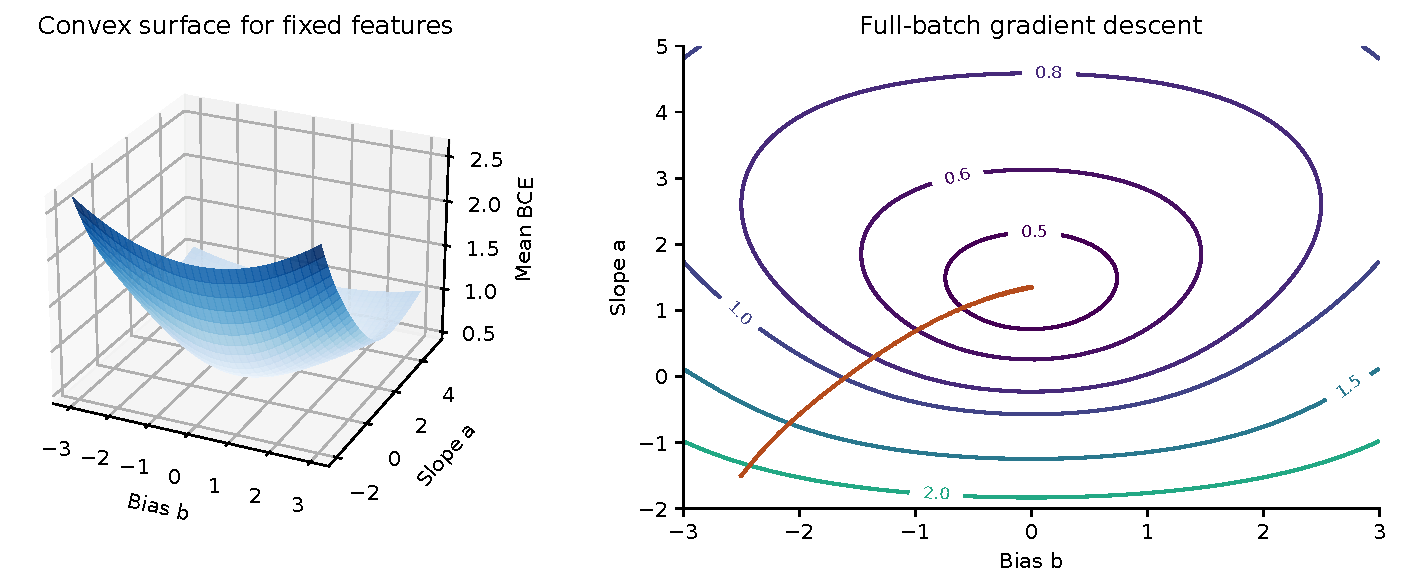
\includegraphics[width=\linewidth]{logreg_1_1/optimization.pdf}
\caption{Mean BCE for a nonseparable one-feature dataset, with bias and slope as
the two axes. The contour plot shows gradient descent from $(-2.5,-1.5)$.
The surface and the contours describe the same objective in parameter space,
not the decision boundary in input space.}
\end{figure}

\subsection{Computational complexity: what exactly is being computed?}
For dense data with $N$ observations and $d$ raw features:
\begin{center}
\begin{tabular}{lll}
\toprule
Operation & Output & Time \\
\midrule
Augmented matrix--vector product $Xw$ & $N$ logits & $\Theta(N(d+1))$ \\
Elementwise sigmoid & $N$ probabilities & $\Theta(N)$ \\
Loss terms and reduction, given logits & One scalar & $\Theta(N)$ \\
Gradient product $X^\top(p-y)$ & $d+1$ derivatives & $\Theta(N(d+1))$ \\
\bottomrule
\end{tabular}
\end{center}
So computing BCE \emph{from raw inputs and weights} is $\Theta(Nd)$ for $d\geq1$.
If probabilities have already been computed and the question only counts the
loss reduction, it is $\Theta(N)$. A full-batch gradient step is also
$\Theta(Nd)$; $T$ steps cost $\Theta(TNd)$. We treat scalar arithmetic and
transcendental functions as constant-cost operations in this usual model.

Storing dense $X$ costs $\Theta(Nd)$ memory, and vectorized predictions need
$\Theta(N)$ additional memory. Minibatches can reduce the working prediction
storage to $\Theta(B)$; streaming avoids storing the full dataset. Sparse matrix
products can cost $\Theta(\operatorname{nnz}(X)+N)$ instead. Explicitly forming
a dense Hessian costs $O(Nd^2)$ time and $O(d^2)$ extra space, which explains why
first-order methods are attractive when $d$ is large.

\subsection{Numerical stability: evaluate the mathematical quantity safely}
The direct expression $-y\log\sigma(z)-(1-y)\log(1-\sigma(z))$ is fragile in
floating point. A large positive score can round $\sigma(z)$ to one, and then
$\log(1-p)$ becomes $\log0$. Large negative scores can overflow $e^{-z}$.
These are numerical failures, not infinite mathematical losses at finite $z$.

Use identities before computing. Since
\[
\log\sigma(z)=z-\log(1+e^z),\qquad
\log(1-\sigma(z))=-\log(1+e^z),
\]
substitution into BCE yields
\begin{equation}
\ell(z,y)=\log(1+e^z)-yz
=\operatorname{softplus}(z)-yz.
\label{eq:lr11-softplus}
\end{equation}
A stable softplus is
$\max(z,0)+\log(1+e^{-|z|})$. For binary labels an even cleaner form is
\[
\boxed{\ell(z,y)=\log\bigl(1+e^{(1-2y)z}\bigr)
=\operatorname{softplus}(-t z),\quad t=2y-1.}
\]
The scalar $tz$ is the signed margin: a large positive margin means confidently
correct, a negative margin means wrong. NumPy's \texttt{logaddexp(0, u)} computes
$\log(1+e^u)$ stably. The signed-margin form also avoids subtracting two large
nearly equal numbers for a correctly classified positive example.

\begin{lstlisting}
import numpy as np

def sigmoid(z):
    z = np.asarray(z, dtype=float)
    return np.exp(-np.logaddexp(0.0, -z))

def loss_and_gradient(X, y, w):
    # X: (N, d+1), y: (N,), w: (d+1,)
    z = X @ w
    loss = np.logaddexp(0.0, (1.0 - 2.0*y)*z).mean()
    gradient = X.T @ (sigmoid(z) - y) / len(y)
    return loss, gradient
\end{lstlisting}

At $z=-1000,y=1$, the loss is approximately $1000$, not a NaN. Clipping
probabilities to $[\varepsilon,1-\varepsilon]$ can prevent a log failure, but
changes the objective near endpoints and can make a stated gradient inconsistent
with that clipped objective. Computing from logits is preferable when available.
Keep $y$ one-dimensional with the code above: mixing shape $(N,1)$ labels and
$(N,)$ probabilities can accidentally broadcast to an $(N,N)$ array.

\subsection{Worked robotics setup: grasp success, cost, and evaluation}
We now connect the equations to an entire modeling workflow. Suppose a robot
uses two nonnegative measurements: centering error $e$ in millimeters and angular
error $\theta$ in degrees. For an interpretable synthetic example, assume the
true conditional success probability is
\begin{equation}
q(e,\theta)=\sigma(3-0.25e-0.08\theta).
\label{eq:lr11-robot}
\end{equation}
These coefficients are illustrative, not measured hardware parameters. Real
success also depends on object geometry, friction, contact, and perception.
The model says that one extra millimeter multiplies success odds by
$e^{-0.25}\approx0.779$, while one extra degree multiplies them by
$e^{-0.08}\approx0.923$, holding the other feature fixed.

At $e=4,\theta=10$, the logit is $1.2$ and $q\approx0.7685$. At
$e=8,\theta=20$, it is $-0.6$ and $q\approx0.3543$. With equal error costs, the
success boundary is
\[
0.25e+0.08\theta=3.
\]
This line is a contour of equal probability, not a physical law of grasping.

\paragraph{Derive the action threshold from consequences.}
Suppose accepting a grasp that fails costs $C_{\mathrm{FP}}$, while rejecting a
grasp that would succeed costs $C_{\mathrm{FN}}$. Assume the two correct decisions
have zero cost. Given a success probability $p$, the expected costs are
\[
\text{accept: }C_{\mathrm{FP}}(1-p),\qquad
\text{reject: }C_{\mathrm{FN}}p.
\]
Accept if the first is smaller, giving
\begin{equation}
p\geq\tau=\frac{C_{\mathrm{FP}}}{C_{\mathrm{FP}}+C_{\mathrm{FN}}},\qquad
z\geq\log\frac{\tau}{1-\tau}.
\label{eq:lr11-cost}
\end{equation}
With $C_{\mathrm{FP}}=8$ and $C_{\mathrm{FN}}=1$, $\tau=8/9\approx0.8889$
and the score threshold is $\log8\approx2.0794$. Equation~\eqref{eq:lr11-robot}
then permits acceptance only when
\[
0.25e+0.08\theta\leq3-\log8\approx0.9206.
\]
The earlier $0.7685$ example would pass a $0.5$ rule but fail this cost-sensitive
rule. The probability model has not changed; the action criterion has.
In deployment this rule relies on useful probability estimates and appropriate
costs. It is not a safety guarantee.

\paragraph{A complete reproducible experiment.}
The companion script generates 1,200 trials using seed 7, with independent
$e\sim U(0,20)$, $\theta\sim U(0,40)$ and
$Y\mid e,\theta\sim\operatorname{Bern}(q(e,\theta))$. It randomly splits them
into 720 training, 240 validation, and 240 test observations. This random split
is appropriate for this independently generated simulation. On real robot
logs, split by object, session, or time as appropriate so near-duplicate frames
and trials do not leak across sets.

Compute each feature's mean $\mu_j$ and standard deviation $s_j$ on the training
set only. Transform all sets using $u_j=(x_j-\mu_j)/s_j$ and prepend the bias
column. Fit the standardized logistic model using full-batch gradient descent
and a fixed illustrative slope penalty $\lambda=0.02$. The script uses the
curvature bound above to choose a conservative step size, with 1,800 updates.
A practical study would select the penalty using validation data too.

Standardization changes coordinates, not the expressive family. If the learned
score is $b_s+\sum_j a_{s,j}(x_j-\mu_j)/s_j$, its physical-unit coefficients are
\[
a_j=\frac{a_{s,j}}{s_j},\qquad
b=b_s-\sum_j\frac{a_{s,j}\mu_j}{s_j}.
\]
However, an $L^2$ penalty in standardized coordinates does change the implicit
penalty on physical-unit coefficients. This is one reason scaling is a modeling
choice as well as a numerical convenience.

\begin{figure}[htbp]
\centering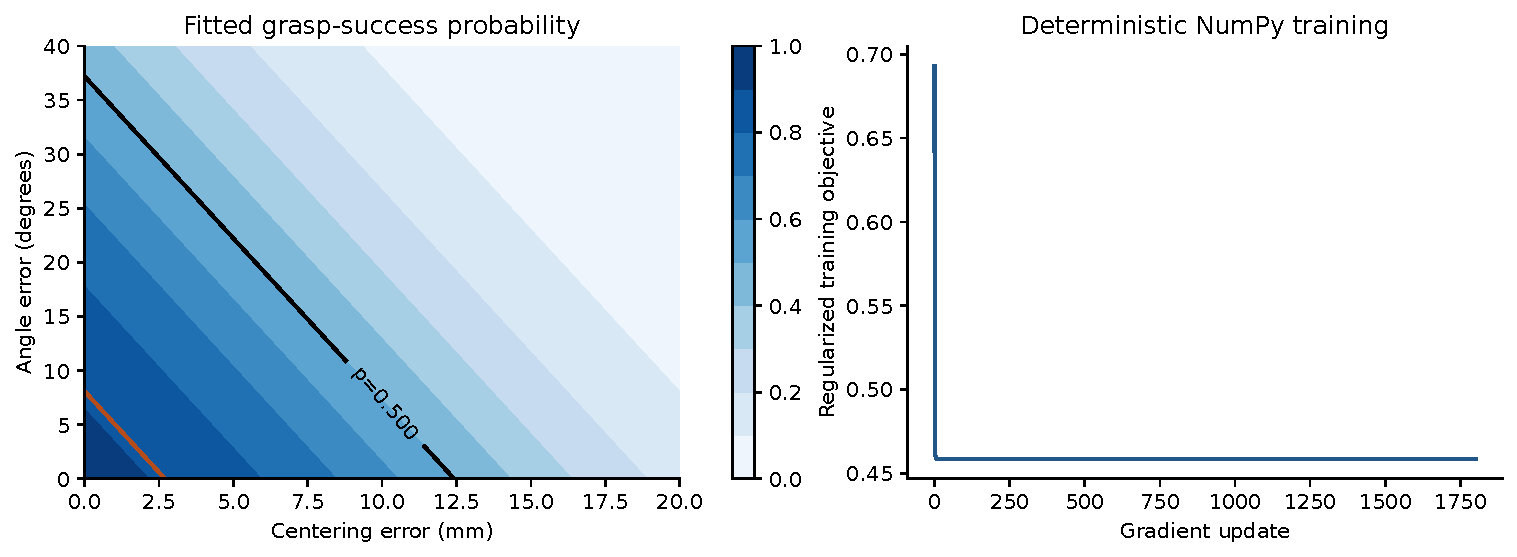
\includegraphics[width=\linewidth]{logreg_1_1/robot_grasp.pdf}
\caption{Synthetic robot experiment. Left: the fitted success field in physical
units, with the $0.5$ and $8/9$ thresholds. Right: the regularized training
objective decreases under the chosen full-batch step size.}
\end{figure}

\paragraph{Evaluate probabilities and decisions separately.}
Report unpenalized test BCE to measure probability quality, accuracy for a stated
threshold, and empirical decision cost for the actual action criterion.
A reliability diagram groups predicted probabilities into bins and compares
each bin's mean probability with its observed success frequency. Small bins are
noisy; an apparent deviation from the diagonal is not automatically systematic
miscalibration. The script records each bin's sample count.

The script also selects a threshold from $0.05,0.06,\ldots,0.95$ using validation
cost alone, then evaluates it on the test data. An empirically selected threshold
can differ from $8/9$ because of finite samples and imperfect probabilities.
Do not select it by looking at test results: the test set is for the final
assessment. For this seeded run the unpenalized test BCE is $0.4317$ nats and accuracy
at $0.5$ is $80.0\%$. The validation-selected threshold is $0.84$.
\begin{center}
\begin{tabular}{lr}
\toprule
Decision threshold & Mean test cost \\
\midrule
$0.5$ & $0.7542$ \\
$8/9$ (cost-derived) & $0.3250$ \\
$0.84$ (validation-selected) & $0.3708$ \\
\bottomrule
\end{tabular}
\end{center}
Here validation tuning does not beat the cost-derived threshold on the test
sample. This is a useful reminder that selecting a threshold on a finite
validation set is itself an estimation problem.
The full numerical output is in the adjacent \texttt{results.json};
all reported quantities can be regenerated from the code.

\begin{figure}[htbp]
\centering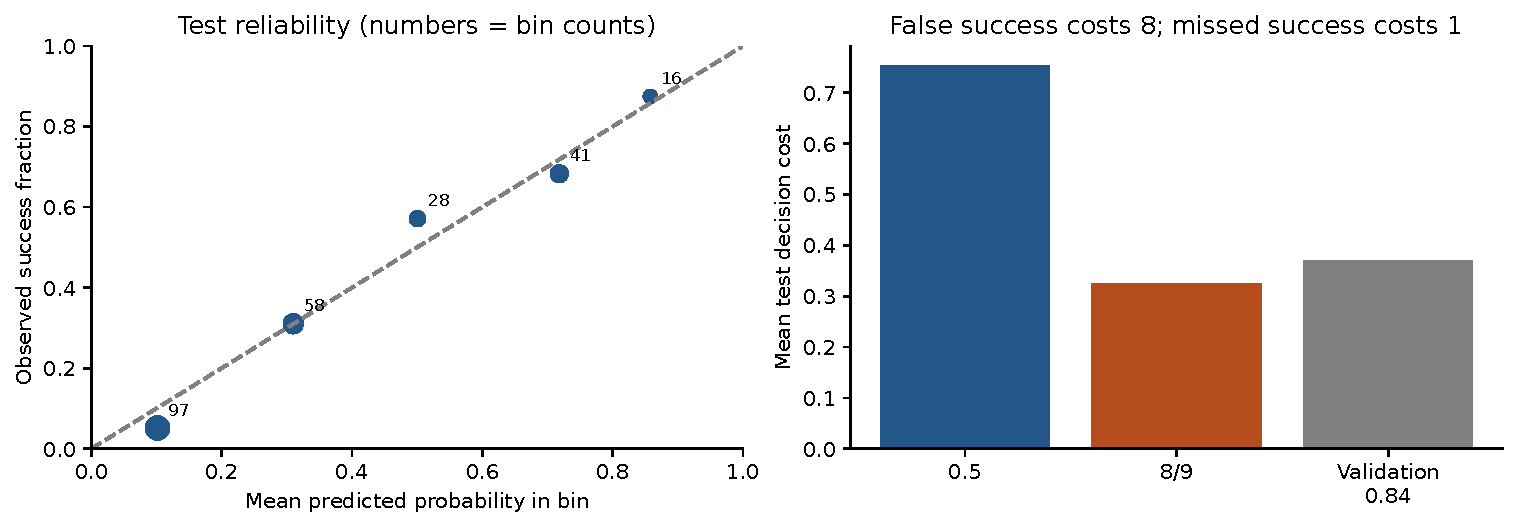
\includegraphics[width=\linewidth]{logreg_1_1/evaluation.pdf}
\caption{Held-out assessment for synthetic grasp trials. Left: a reliability
diagram, with counts showing how much evidence supports each bin. Right: mean
cost at a default threshold, the analytically derived cost threshold, and a
validation-selected threshold. These are one simulation's measurements, not
claims of general superiority or hardware performance.}
\end{figure}

\paragraph{What would break this setup?}
A new gripper or different object material can change $q(x)$ even when the two
features look familiar. Missing interactions may make affine log-odds inadequate.
Selection bias arises if training only records grasps the old policy chose to
attempt; rejected grasps may have no observed outcome. Label errors, rare
failures, correlated trials, and feature drift also matter. More confident
numbers alone solve none of these problems. The model's meaning is conditional
on its observations, data collection, and deployment distribution.

\subsection{From-scratch practice and checks}
The executable companion is
\texttt{deep\_learning/code/logreg\_1\_1.py}. It uses NumPy for the model and
optimization, and Matplotlib for figures; it uses no machine-learning library.
Run it from the repository root:
\begin{lstlisting}[language=bash]
python deep_learning/code/logreg_1_1.py
make dl
\end{lstlisting}
It regenerates seven vector-PDF figures and a JSON result summary in
\path{deep_learning/figures/logreg_1_1/}. The chapter can be compiled with
the committed figures without running Python. The full script includes an
$L^2$-regularized objective, training, data splitting, standardization, evaluation,
and the following meaningful numerical checks:
\begin{enumerate}
\item Compare the analytic gradient against centered finite differences,
$[J(w+\varepsilon e_j)-J(w-\varepsilon e_j)]/(2\varepsilon)$.
\item Check the Hessian's eigenvalues on a small dataset and verify that the
chosen full-batch updates do not increase the regularized objective.
\item Evaluate extreme logits $\pm1000$ and require finite losses and probabilities.
\item Check $\sigma(0)=1/2$ and $\sigma(-z)=1-\sigma(z)$.
\end{enumerate}
These checks catch implementation mistakes; they do not replace the mathematical
proofs or establish generalization to a robot.

\paragraph{Suggested implementation order.}
First reproduce the two-point hand update using only arrays. Then implement
stable sigmoid and BCE, verify the gradient numerically, add repeated updates,
and plot the training loss. Only after that add standardization, a validation
split, and decision costs. Predict what each change should do before running it.
This makes the code an experiment on the mathematical ideas rather than a recipe.

\subsection{Reasoning exercises}
Try these before reading the worked answers below. They are independent of the
main derivation, so the conceptual narrative need not be interrupted.
\begin{exercise}[Same classes, different probabilities]
For $w=(-3,1,1)^\top$, compare $w$ and $10w$ at $(1,2)$ and $(2,2)$.
Do the boundaries, hard predictions, and losses for a positive label agree?
\end{exercise}
\begin{exercise}[Recover a probability model]
An intercept-only dataset contains 20 successes and 30 failures. Derive the
maximum-likelihood probability and intercept. What happens if all 50 succeed?
\end{exercise}
\begin{exercise}[Costs change a boundary]
A classifier has score $z=-3+x_1+x_2$. Derive the action boundary when a false
positive costs nine times a false negative. Which side predicts one?
\end{exercise}
\begin{exercise}[Feature maps and convexity]
Use features $(x_1,x_2,x_1x_2)$ to express XOR on $\{-1,1\}^2$. Explain why the
training objective is convex in its coefficients, despite the nonlinear boundary.
Would the same proof apply if the features were outputs of a trained hidden layer?
\end{exercise}
\begin{exercise}[Complexity and data shape]
For $N=10^6$ and $d=100$, identify the dominant forward-pass operation. Explain
why storing labels as $(N,1)$ while predictions have shape $(N,)$ is dangerous.
How does a batch of size $B$ change working memory and per-step time?
\end{exercise}

\subsection{Worked answers and conceptual checkpoints}
\paragraph{1. Scaling.}
At $(1,2)$, both logits are zero and both probabilities are $0.5$. At $(2,2)$,
the logits are $1$ and $10$, with probabilities about $0.7311$ and $0.99995$.
Positive-label losses are $\log(1+e^{-1})\approx0.3133$ and
$\log(1+e^{-10})\approx0.0000454$. Boundaries and hard classes agree. If the
label at $(2,2)$ were zero instead, the larger scale would be far more costly:
about $10.00005$ versus $1.3133$. Confidence has consequences.

\paragraph{2. Intercept-only estimation.}
The loss is $-0.4\log p-0.6\log(1-p)$; differentiating gives the minimum
$p=0.4$. Thus $b=\log(0.4/0.6)=\log(2/3)\approx-0.4055$. If all labels are one,
the loss decreases as $b\to+\infty$, and no finite unregularized optimum exists.

\paragraph{3. Costs.}
The threshold is $\tau=9/10$, so the logit threshold is $\log9$. The new boundary
is $x_1+x_2=3+\log9\approx5.1972$, with class one on the greater-than side.
It is parallel to the equal-cost boundary and requires stronger evidence.

\paragraph{4. Fixed features.}
Take zero bias and zero coefficients on $x_1,x_2$, with coefficient $-k$ on
$x_1x_2$, $k>0$. The four signed scores have the required signs. The Hessian
proof applies to the resulting fixed design matrix. With a trainable hidden
layer, the feature matrix itself depends on parameters, and the positive
semidefinite form above is no longer the full Hessian.

\paragraph{5. Computation.}
The dense product $Xw$ uses roughly $N(d+1)$ multiply--accumulate operations,
about $10^8$ here. Broadcasting $(N,)$ minus $(N,1)$ can create an $(N,N)$ array,
which is both mathematically wrong and enormous. A dense batch step costs
$\Theta(Bd)$ time and stores $\Theta(Bd)$ feature entries if batches are streamed,
plus parameters and $\Theta(B)$ temporary predictions. An epoch still processes
$N$ observations and costs $\Theta(Nd)$.

\begin{keyidea}[Reconstruct the method from its meaning]
An affine score describes additive log-odds. The sigmoid converts that evidence
into a Bernoulli probability. Independence turns observed-label probabilities
into a product likelihood, and the negative logarithm turns that product into
an additive loss. The gradient $X^\top(p-y)/N$ adjusts evidence according to
probability errors. Convexity follows from nonnegative Bernoulli variances, but
finite solutions require more than convexity. Finally, the decision threshold
comes from the consequences of actions, not from the probability model alone.
\end{keyidea}

\paragraph{Scope and reading.}
This section expands the supplied lecture excerpts (slides 5--10 and their
questions). Section 1.2 can develop entropy, KL divergence, and maximum likelihood
more generally; the later sections can reinterpret the same affine--sigmoid
computation as a neural-network unit. General background texts already present
in this repository include \citet{bishop2006pattern} and
\citet{goodfellow2016deep}. All plots in this section are generated by its companion
script from explicit formulas or synthetic data.
